\documentclass[14pt]{extreport}
\usepackage{gost}

\begin{document}

\pagestyle{empty} %  выключаем нумерацию
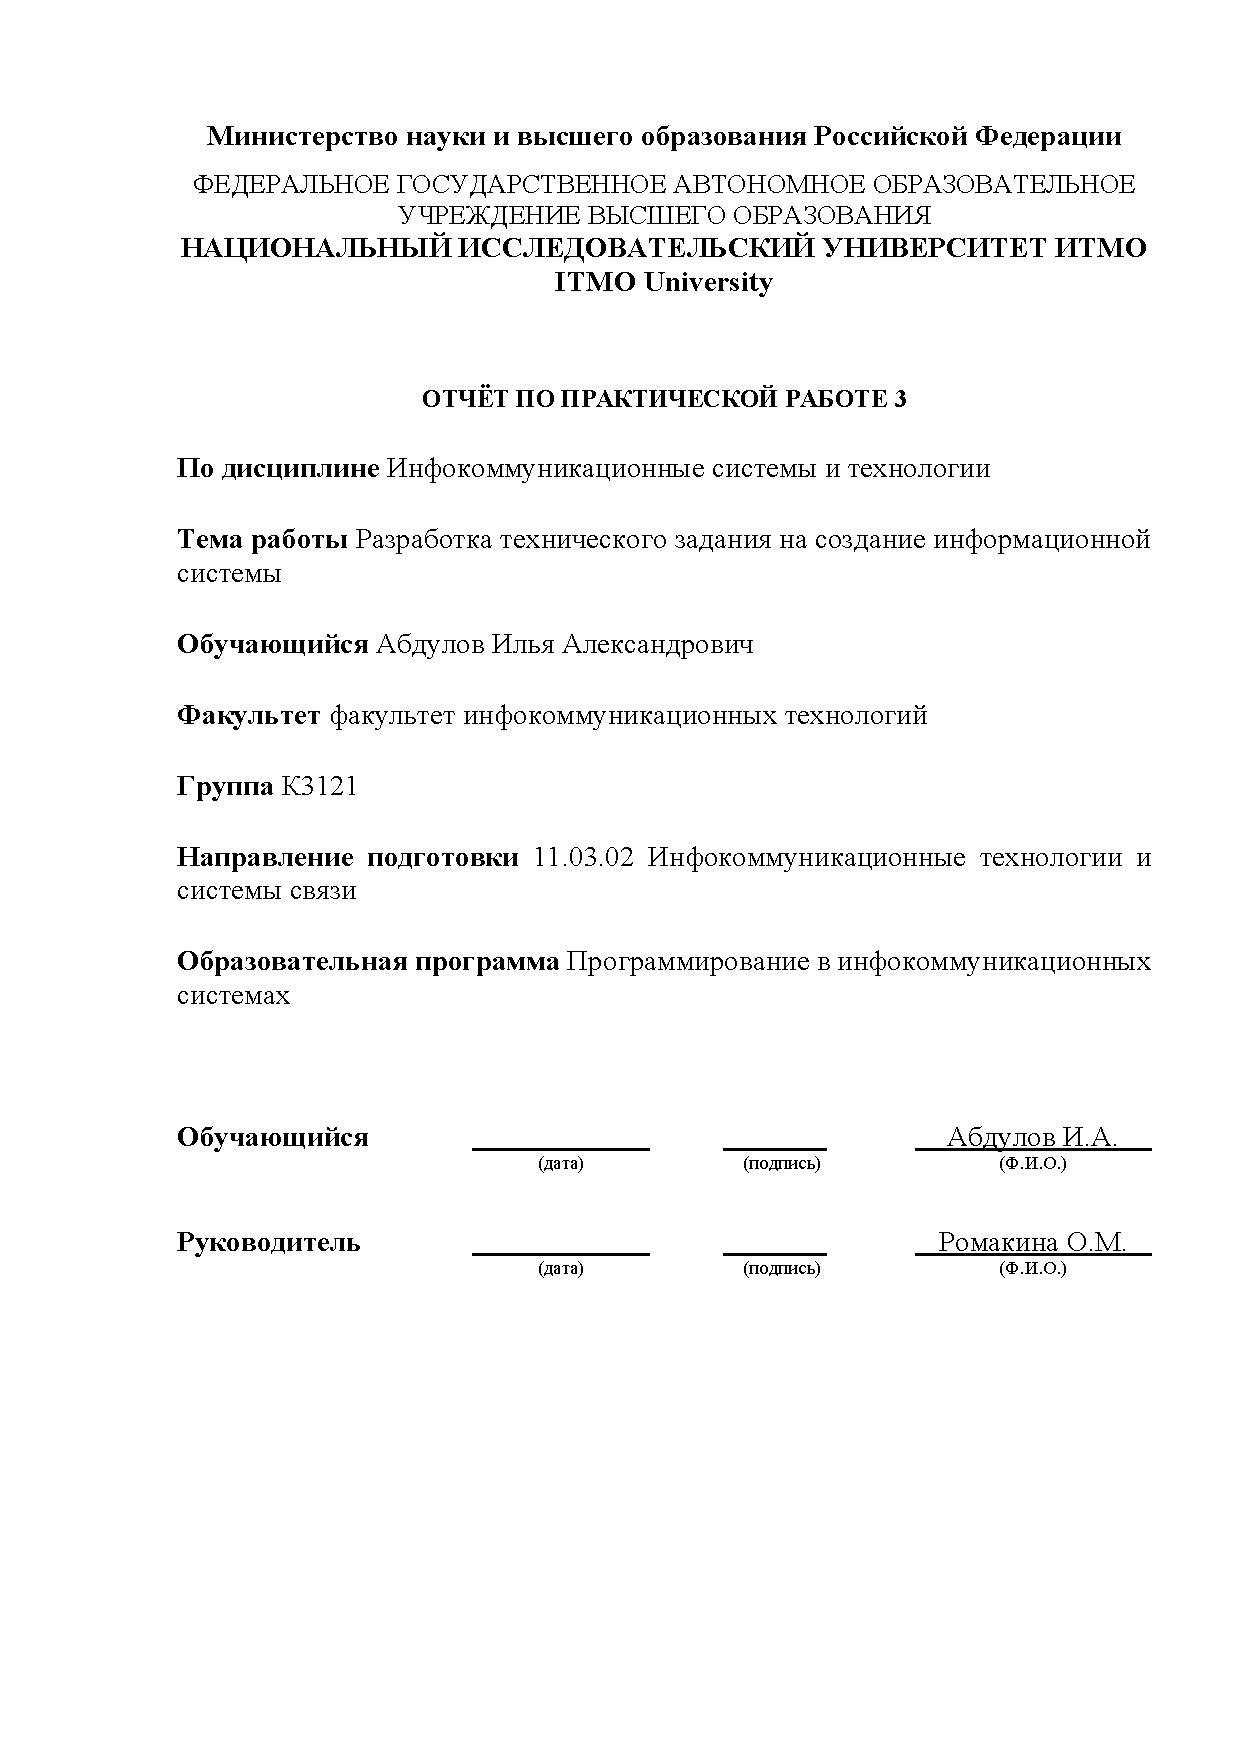
\includepdf[pages=-,pagecommand={}]{titulCourse.pdf}
\pagestyle{plain} % включаем нумерацию

\chapter{Базы данных. Занятие 1-2 (09.03.2023)}

\section{Эссе}

Тема задания: В каких сферах жизни человек может столкнуться с БД? В каких сферах образования используются базы данных? Какие возможности дает использование БД? Какие риски могут подкарауливать пользователей БД?

База данных — это совокупность структурированных сведений, относящихся к определённой теме или задаче, организованная таким образом, чтобы обеспечить удобное представление этой совокупности, как в целом, так и в любой ее части. Базы данных позволяют безопасно записывать, извлекать, хранить очень большие объемы структурированных данных.

База данных обычно управляется системой управления базами данных (СУБД). СУБД позволяет получать, обновлять, упорядочивать, оптимизировать, резервировать и восстанавливать информацию, хранящуюся в базе данных.

Базы данных сейчас используются почти во всех сферах жизни человека. Например, в социальных сетях и блогах требуется хранить данные о пользователе: логин, пароль, контактный телефон, электронную почту, дату рождения и т.д. Также базы данных используются на сайтах, чтобы хранить и извлекать контент, наполнение страниц сайта. То есть пользователь при обращении к сайту получает на свое устройство сведения из баз данных.

Базы данных активно используются в сфере образования. В данной сфере информационных данных огромные объемы и их требуется где-то хранить. Базы данных используются для составления расписания занятий конкретного пользователя в образовательном учреждении, для хранения информации о обучающихся в образовательном учреждении, для ведения журналов посещаемости и успеваемости обучающихся.

Использование БД предоставляет много возможностей. Все нужные данные можно быстро найти в большом количестве информации. Данные можно быстро добавлять и обновлять. Также база данных дает возможность сохранять очень большие объемы данных — миллионы различных записей.

В то же время при использовании баз данных пользователей системы могут подкарауливать некоторые риски. Главным риском является безопасность БД и СУБД. Базы данных должны иметь уровни защиты и ограничения от несанкционированного доступа, так как иногда в БД хранится конфиденциальная информация, например, паспортные данные человека. Кроме того, БД должны быть восстанавливаемы, потому что иногда происходят аппаратные сбои, что может привести к потере или смене данных.

\section{Кейс}

Тема задания: Опишите Ваш день: где и как Вы используете БД? 

Я встречаюсь с базами данных ежедневно, даже не задумываясь об этом. Ведь практически все приложения, которыми мы пользуемся в наших смартфонах или других устройствах используют базы данных.

Первым делом рано утром я проверяю приложение my.itmo, чтобы посмотреть какие пары сегодня стоят в расписании. Расписание занятий содержится в БД, к которой я обращаюсь при просмотре расписания. Также базы данных содержат информацию о моем аккаунте в my.itmo, в соответствии с чем выводится именно мое расписание.

Также, утром я проверяю свою социальную сеть VK на наличие новостей и сообщений. Информация о моем аккаунте в социальной сети и контент, которым наполнена соцсеть, содержится в базах данных, к которым я обращаюсь при использовании приложения.

Чтобы добраться до университета я использую метро или автобус, в котором прикладываю свой БСК для считывания системой. Система контроля проездных обращается к базе данных, которая проверяет, действителен ли мой БСК, и регистрирует очередную поездку в транспорте в базе данных.

Когда я приезжаю в университет, чтобы войти мне нужно приложить свой студенческий пропуск к турникету, который считает номер моего пропуска и обратится к базе данных вуза для проверки наличия данного ID пропуска среди всех допустимых ID.

В перерыве между занятиями я открываю мессенджер Telegram, чтобы проверить чаты и сообщения. В это время я обращаюсь к базе данных, которая относится к моему аккаунту в мессенджере.

Ежедневно мы обращаемся к базам данных десятки раз, сами того не зная. Благодаря им, мы можем работать и получать большие объемы данных, которые используются нами для различных целей в цифровых устройствах. Без баз данных не существовали бы те технологии, которыми мы постоянно пользуемся.


\end{document}